\documentclass[twocolumn]{article}

\usepackage{graphicx}
\usepackage{amsmath}
\usepackage{amsthm}
\usepackage{amssymb}
\usepackage{url}
\usepackage{multirow}
\usepackage{times}
\usepackage{fullpage}
\usepackage{algorithm}
\usepackage{algpseudocode}
\newcommand{\comment}[1]{}
\algrenewcommand{\algorithmicrequire}{\textbf{Input:}}
\algrenewcommand{\algorithmicensure}{\textbf{Output:}}
\algrenewcommand{\algorithmicforall}{\textbf{for each}}

\title{CS618: Group xx \\ Project Report}
\author{
\begin{tabular}{c   c}
	Proneet Verma & Saurav Kumar \\
	Student ID 44 & Student ID 45 \\
	Roll Number 12520 & Roll Number 12641 \\
	\url{proneetv@iitk.ac.in} & \url{ksaurav@iitk.ac.in} \\
	Dept. of MSE & Dept. of CSE \\
	\multicolumn{2}{c}{Indian Institute of Technology, Kanpur}
\end{tabular}
}
\date{Initial Report \\	% replace by ``initial'' or ``final'' as appropriate
\today}	% replace by actual date of submission or \today

\begin{document}
\maketitle
\begin{abstract}
	%
	B+ Trees are efficient and effective in indexing data stored in databases. This project aims to efficiently \mbox{implement} and analyze performance of general queries in B+ Trees distributed over a multi-node computer network. We plan to consider several factors for \emph{data \mbox{distribution} among servers}, such as geographical location of the node, \mbox{bandwidth} of network connecting the root and the node, hardware configuration of the node, and \emph{likelihood of data} being queried in order to arrive at a \mbox{comprehensive analysis.} 
	%
\end{abstract}

\section{Introduction and Problem Statement}

% State the problem as clearly and as formally as possible.  Explain the
% notations, etc.  Explain the objectives, and all the inputs.  If possible,
% motivate why this is an interesting problem.
The problem consists of 2 parts:
\begin{itemize}
\item Implementation of distributed database which uses B+ Tree to efficiently index the database
\item Analysis of response time on general queries
\end{itemize}
\begin{figure}[h]
	\centering
	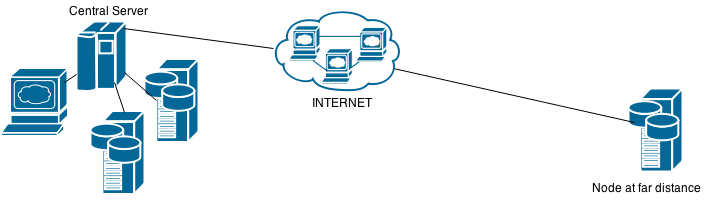
\includegraphics[width=0.95\columnwidth]{dbpt.png}
	\caption{Distributed Database}
	\label{fig:block}
\end{figure}

\textbf{Score based system}: For this problem, we will use a score-based technique to distribute data among the nodes. Servers will have their scores computed based on their average response time which depends on network response time, processing speed and Disk I/O time. This score will roughly determine how much data should be kept on which servers.

\textbf{Likelihood}: Since some data (keys) may be returned more often than others depending on distribution of data and query responses, we will try to find an optimum strategy to keep more frequent data in servers with better score. To test the effectiveness of the strategy we will train the model with some distribution of queries and test with same distribution of query data. For actual practise, we propose online migration of nodes between servers based on query and response analytics
\subsection{Related Material}

% Fill in all relevant work, datasets, websites, etc.
http://dl.acm.org/citation.cfm?id=1566451
\comment{

Can also comment out paragraphs, etc.

}

\section{Algorithm or Approach}

% Details of the method.
% Put in a pseudo-code, etc. if applicable.

\comment{

\begin{algorithm}[t]
	\caption{Indexing}
	\label{alg:indexing}
	\begin{algorithmic}[1]
		\Require Database $D$, Query $Q$
		\Ensure Result set $A$
		\State $A \gets$ Search($Q$, $D$)
		\State \Return $A$
	\end{algorithmic}
\end{algorithm}

And refer as Algorithm \ref{alg:indexing}.

}

% Explain with figures.

\comment{

Use the following format for figures:

\begin{figure}[t]
	\centering
	\includegraphics[width=0.95\columnwidth]{figure_file}
	\caption{This figure explains this.}
	\label{fig:block}
\end{figure}

And refer as Figure \ref{fig:block}.

}

\section{Results}

% Details of results, in tabular and/or graphical formats.

% More importantly, analyze the results.

\comment{

\begin{table}[t]
	\centering
	\begin{tabular}{|c||cc|}
		\hline
		Header 1 & Desc 1 & Desc 2 \\
		\hline
		\hline
		Row 1 & Data 1-1 & Data 1-2 \\
		Row 2 & Data 2-1 & Data 2-2 \\
		\hline
	\end{tabular}
	\caption{Table of results.}
	\label{tab:results}
\end{table}

And refer as Table \ref{tab:results}.

}

\section{Conclusions}

% Clearly state the conclusions.
% Outline the future work.

\section*{References}

% Directly type in bib entries.

% Better is to use \emph{bibtex}.

\end{document}

